\chapter{Quantum Preconditioning}\label{ch:sec07}

Consider the elliptic problem $-\operatorname{div}(A\nabla u) = f$, with weak form
\begin{equation}
  a(u, v) = \int_D A\nabla u \cdot \nabla v\,\dd x, \qquad
  \alpha\abs{\eta}^2 \le \eta \cdot A\eta \le \beta\abs{\eta}^2,
\end{equation}
and Galerkin formulation $a(u, v) = f(v)$ for $v \in H_0^1(\Omega)$. With
$H^2$ regularity, $\norm{u - u_h} \le C_{A, f}\, h$.

Let $\lambda_1, \dots, \lambda_N$ be a basis of $V_h$, with
$N = \dim V_h = (2^\ell - 1)^d$. Writing $c = (c_1, \dots, c_N)^{\mathsf{T}}$ and
$u_h = \sum_{j=1}^N c_j \lambda_j$, the stiffness system is
\begin{equation}
  S c = r, \qquad S = (a(\lambda_j, \lambda_k))_{j,k=1}^N, \qquad
  r = ((f, \lambda_j)_{L^2})_{j=1}^N.
\end{equation}

\section{Block encoding}\label{sec:sec07-block}

A block encoding of $S$ is a unitary of the form
\begin{equation}
  U_S = \begin{pmatrix} \tfrac{1}{\gamma} S & * \\ * & * \end{pmatrix},
\end{equation}
where $\gamma > 0$ is a normalization constant chosen so that the spectral norm of
$\tfrac{1}{\gamma}S$ is bounded by $1$. Then
$S = \gamma(\bra{0} \otimes I_d) U_S (\ket{0} \otimes I_d)$, with the operational
effect
\begin{equation}
  (\bra{0} \otimes I_d) U_S \ket{0}\ket{i} = \frac{1}{\gamma} S\ket{i},
\end{equation}
since $\bra{0} \otimes I_d = (I\ \ 0)$, $\ket{0} \otimes I_d = \begin{psmallmatrix} I \\ 0 \end{psmallmatrix}$, and
$(I\ \ 0)\begin{psmallmatrix} S/\gamma & * \\ * & * \end{psmallmatrix}\begin{psmallmatrix} I \\ 0 \end{psmallmatrix} = \tfrac{1}{\gamma}S$.

\begin{definition}[Projection as a $C_\Pi$NOT gate]
Let $N, m \in \N$ with $N \le 2^m$, and let $\Pi : \C^{2^m} \to \C^N$ be a
projection, i.e.\ a matrix with orthonormal rows. We call a gate on $m + 1$
qubits a $C_\Pi$NOT gate if it flips the last bit iff the first $m$ bits represent
a vector in $\operatorname{Range}(\Pi)$:
\begin{equation}
  \Pi\dg\Pi \otimes (\ket{0}\bra{1} + \ket{1}\bra{0}) + (I - \Pi\dg\Pi) \otimes I_d.
\end{equation}
\end{definition}

\begin{example}
Consider the projection $\Pi : \C^{2^m} \to \C^{2^{m-1}}$ of a vector of length
$2^m$ onto its first half, $x \mapsto (x_0, \dots, x_{2^{m-1}-1})^{\mathsf{T}}$.
\end{example}

\begin{definition}[Block encoding, normalization, and subnormalization]
Let $N_1, N_2, m \in \N$ with $N_1, N_2 \le M := 2^m$. Let $S \in \C^{N_2 \times N_1}$
and $\gamma \ge \norm{S}$. Further let $\Pi_1 : \C^M \to \C^{N_1}$ and
$\Pi_2 : \C^M \to \C^{N_2}$ be projections. Consider a quantum algorithm
implementing a unitary matrix $U_S \in \C^{M \times M}$ together with
implementations of a $C_{\Pi_1}$NOT and a $C_{\Pi_2}$NOT gate. We call
$(U_S, C_{\Pi_1}\mathrm{NOT}, C_{\Pi_2}\mathrm{NOT})$ a block encoding of $S$ if
\begin{equation}
  \gamma\,\Pi_2 U_S \Pi_1\dg = S.
\end{equation}
The normalization factor is $\gamma(U_S) := \gamma$, and the subnormalization
factor is $\tilde{\gamma}(U_S) := \tfrac{\gamma(U_S)}{\norm{S}} \ge 1$ (with
$\norm{\cdot}$ the spectral norm).
\end{definition}

\begin{remark}
The upper-left $M \times M$ block $\hat{S}$ of the unitary
$U_{\hat{S}} := C_{\Pi_2}\mathrm{NOT}\,(U_S \otimes I_d)\,C_{\Pi_1}\mathrm{NOT} \in \C^{2M \times 2M}$
is equivalent to $S$ in the sense $\hat{S} = \Pi_2\dg S \Pi_1$.
\begin{itemize}
  \item $\tilde{\gamma}(U_S)$ measures the extent to which the norm of a vector is
    preserved under the action of the block encoding.
  \item The computational complexity of solving a linear system is proportional to
    $\tilde{\gamma}(U_S)\cdot\kappa(S)$, and not just $\kappa(S)$.
  \item $\kappa(A) = \norm{A}\norm{A\dg} = \sigma_{\max}(A)/\sigma_{\min}(A)$.
\end{itemize}
\end{remark}

\begin{proposition}[Operations on block-encoded matrices]
Let $A \in \C^{m_A \times n_A}$ and $B \in \C^{m_B \times n_B}$ with block
encodings $(U_A, C_{\Pi_{A,1}}\mathrm{NOT}, C_{\Pi_{A,2}}\mathrm{NOT})$ and
$(U_B, C_{\Pi_{B,1}}\mathrm{NOT}, C_{\Pi_{B,2}}\mathrm{NOT})$. Then block encodings
with normalization $\gamma$ and subnormalization $\tilde{\gamma}$ can be
constructed for the following operations:
\begin{align}
  A \otimes B &: \gamma = \gamma(U_A)\gamma(U_B),\quad \tilde{\gamma} = \tilde{\gamma}(U_A)\tilde{\gamma}(U_B); \\
  A\dg &: \gamma = \gamma(U_A),\quad \tilde{\gamma} = \tilde{\gamma}(U_A); \\
  \begin{psmallmatrix} A & 0 \\ 0 & B \end{psmallmatrix} &: \gamma = \max\{\gamma(U_A), \gamma(U_B)\},\quad \tilde{\gamma} = \max\{\tilde{\gamma}(U_A), \tilde{\gamma}(U_B)\}; \\
  AB &: \gamma = \gamma(U_A)\gamma(U_B),\quad \tilde{\gamma} \le \begin{cases} \kappa(A)\tilde{\gamma}(U_A)\tilde{\gamma}(U_B) & n_A \ge m_A, \\ \kappa(B)\tilde{\gamma}(U_A)\tilde{\gamma}(U_B) & m_B \ge n_B; \end{cases} \\
  \begin{psmallmatrix} A & B \end{psmallmatrix} &: \gamma = \sqrt{\gamma(U_A)^2 + \gamma(U_B)^2},\quad \tilde{\gamma} \le \sqrt{\tilde{\gamma}(U_A)^2 + \tilde{\gamma}(U_B)^2}; \\
  \mu_A A + \mu_B B &: \gamma = \sqrt{2(\abs{\mu_1}\gamma(U_A) + \abs{\mu_2}\gamma(U_B))}, \quad \mu_A, \mu_B \in \C,
\end{align}
provided the dimensions are compatible (in the sense $\Pi_{B,2} = \Pi_{A,1}$ for
the product, $\Pi_{A,2} = \Pi_{B,1}$ for the concatenation and the sum, and
$\Pi_{A,1} = \Pi_{B,1}$ for the sum). Without further assumptions, the
subnormalization of the sum can be unbounded.
\end{proposition}

\begin{proposition}[Block encoding of block-diagonal matrices]
Let $n, m, N, M \in \N$ with $N = 2^n$ and $M \le 2^m$. Let $\gamma > 0$ and let
$A \in \C^{NM \times NM}$ be an $N \times N$ block-diagonal matrix with blocks of
size $M \times M$. Let $\Pi : \C^{(2^m)} \to \C^M$ be a projection with an
implementation of $C_\Pi\mathrm{NOT}$. Let $U_A$ be a quantum circuit operating on
two qubit registers $\ket{j}_n, \ket{x}_m$, applying a block encoding of the
$j$-th diagonal block $A_{jj}$ with the projection $\Pi$ and normalization
$\gamma$ on the register $\ket{x}$, i.e.\
$\gamma(\bra{j} \otimes \Pi) U_A (\ket{j} \otimes \Pi) = A_{jj}$. Then we can
construct a block encoding of $A$ with normalization $\gamma$; its
subnormalization is the minimum of the subnormalizations over all blocks.
\end{proposition}

\section{The quantum linear system problem}\label{sec:sec07-qlsp}

Consider $S c = r$, and assume $\norm{S} \ge 1$, $\norm{r} \ge 1$, and
$\norm{S^{-1}} = \kappa(S)$.

\begin{definition}[Quantum linear system algorithm]
Let $\kappa \ge 0$ and $\mathrm{tol} > 0$. Consider an algorithm that takes as
input two oracles: $O_S$, which applies a block encoding to a matrix $S$, and
$O_r$, which prepares the state $\ket{r}$. We say that the algorithm solves the
quantum linear system problem for condition $\kappa = s(O_S \norm{S})$ and error
$\mathrm{tol}$ if it produces a state $\ket{\tilde{c}}$ such that
\begin{equation}
  \norm{\ket{\tilde{c}} - \frac{S^{-1}\ket{r}}{\norm{S^{-1}\ket{r}}}} \le \mathrm{tol}.
\end{equation}
The number of calls to each oracle is the query complexity. We also allow the
algorithm to fail with a probability independent of $\kappa$ and $\mathrm{tol}$, in
which case it should communicate the failure via an additional flag bit.
\end{definition}

The HHL algorithm has complexity $\bigo(\kappa^2\,\mathrm{tol}^{-1})$; one can
improve both the $\kappa$ and $\mathrm{tol}$ dependence by variable-time amplitude
amplification, or by constructing $\ket{c}$ directly.

\begin{theorem}[Existence of fast quantum linear system algorithms]
A solution of the quantum linear system problem (in the sense of the definition
above) can be computed with query complexity
$\bigo(\kappa\,\polylog(\kappa\,\mathrm{tol}^{-1}))$.
\end{theorem}

For the measurement, $\braket{c|U|c}$ uses the Hadamard test, $\braket{m|c}$ the
SWAP test, and $\braket{c|A|c}$ a measurement, with cost
$\bigo(\kappa\,\mathrm{tol}^{-1}\polylog(\kappa\,\mathrm{tol}^{-1}))$. For an
elliptic PDE, $\kappa(S) \sim \bigo(h^{-2})$.

\section{Challenges of quantum preconditioning}\label{sec:sec07-challenges}

Consider the preconditioned system $P S P_r\, y = P r$, $c = P_r y$. In sparse
preconditioning, $P$ and $P_r$ are decompositions of linear operators, and one
would like to compute $P S P_r$ via block encoding. However, the spectral norm of
any matrix implemented on a quantum computer is $\le 1$, so multiplying a vector
by a matrix may decrease the norm of the resulting vector; recovering it via
amplitude amplification requires $\bigo(\kappa)$ times. This leads to
$\kappa(P)\kappa(P_r) \propto \kappa(S)$, which results in significant
subnormalization and machine-precision issues.

\section{Optimal multilevel preconditioning}\label{sec:sec07-bpx}

\paragraph{BPX preconditioner.}
Following Bramble, Pasciak, and Xu (\emph{Parallel multilevel preconditioners},
Math.\ Comp.\ 55(191):1--22, 1990),
\begin{equation}
  P_x = \sum_{\ell=1}^L \sum_{j=1}^{\dim V_\ell} 2^{-\ell(d-2)}(u, \lambda_j^{(\ell)})_{L^2}\lambda_j^{(\ell)},
\end{equation}
a hierarchical decomposition of $V_h$ on a hierarchy of grids
$G_1, \dots, G_L$, with $G_\ell$ having $h_\ell = 2^{-\ell}$, $\ell = 1, \dots, L$,
$G_L = G_h$. Consider the finite element spaces
$V_\ell = \operatorname{span}\{\lambda_j^{(\ell)}\}_{j=1}^{\dim V_\ell}$.

\begin{lemma}[Optimality of the BPX preconditioner]
Let $d \in \N$, $D \subset \R^d$ a bounded domain, and
$V_1 \subset \cdots \subset V_L \subset H_0^1(D)$ finite element spaces. If, for
all $1 \le \ell \le L$, these spaces fulfill the Jackson estimates
\begin{equation}
  \inf_{v_\ell \in V_\ell} \norm{u - v_\ell}_{L^2} \le 2^{-\ell}C_1\norm{u}_{H^1}
  \quad \text{for all } u \in H_0^1(D),
\end{equation}
and the Bernstein estimates
\begin{equation}
  \norm{v_\ell}_{H^1} \le 2^\ell C_2\norm{v_\ell}_{L^2}
  \quad \text{for all } v_\ell \in V_\ell,
\end{equation}
with constants $C_1, C_2 > 0$ independent of $\ell$ and $L$, then the condition of
the symmetrically preconditioned stiffness matrix
$\kappa(P^{1/2} S P^{1/2}) = \bigo(1)$ is bounded independent of $L$.
\end{lemma}

Since the preconditioned system $PS$ generally has no bounded condition number,
we actually split the preconditioner $P$, as is done for multilevel frames in the
context of finite element methods. For the split one considers the corresponding
generating system
\begin{equation}
  \mathcal{F} = \{f_{j,\ell} := 2^{-\ell(2-d)/2}\lambda_j^{(\ell)} \mid 1 \le \ell \le L,\ 1 \le j \le \dim V_\ell\}.
\end{equation}
Let $P : \R^{\abs{\mathcal{F}}} \to V_L$ be the linear function given by
$Fc = \sum_{\ell=1}^L \sum_{j=1}^{\dim V_\ell} c_{j,\ell} f_{j,\ell}$. Then
$P = FF^{\mathsf{T}}$, and we obtain the preconditioned system
\begin{equation}
  F^{\mathsf{T}} S F\, y = F^{\mathsf{T}} r, \qquad c = Fy.
  \label{eq:sec07-precond}
\end{equation}

\section{Implementation}\label{sec:sec07-impl}

In addition to the continuous FE spaces $V_\ell$, consider the auxiliary
discontinuous spaces on $G_\ell$ with dimension $2^{d(\ell+1)}$
(\cref{fig:sec07-grid}). For each cell $G_j \in G_\ell$, there are $2^d$ local
orthonormal bases $\psi_{j,1}^{(\ell)}, \dots, \psi_{j,2^d}^{(\ell)}$,
$1 \le j \le 2^{d\ell}$. Let $C_\ell$ be the matrix representation of the gradient
$\nabla : V_\ell \to Q_\ell^d$ (of size $(2^\ell - 1)^d \times d\,2^{d(\ell+1)}$),
and $T_{\ell, L}$ the transfer matrix $Q_\ell \to Q_L$. The vector-valued space
$Q_\ell^d = Q_\ell \otimes \R^d$ has an orthonormal basis
$\psi_{j,k}^{(\ell)} \otimes e_s$.

\begin{figure}[ht]
  \centering
  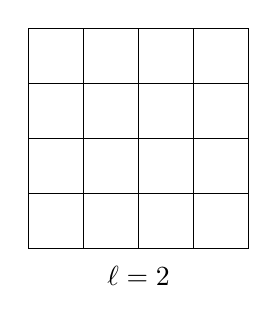
\begin{tikzpicture}[scale=0.7]
    \draw (0,0) grid (4,4);
    \node at (2,-0.5) {$\ell = 2$};
  \end{tikzpicture}
  \caption{An auxiliary discontinuous space on the grid $G_\ell$ for $\ell = 2$.}
  \label{fig:sec07-grid}
\end{figure}

Let $D_A$ be a block-diagonal matrix with $d \times d$ blocks
$(D_A)_{jj} = A|_{T_j}$. Then
\begin{equation}
  S = C_L^{\mathsf{T}}(D_A \otimes I_{d^2}) C_L, \qquad
  F^{\mathsf{T}} S F = C_F^{\mathsf{T}}(D_A \otimes I_{d^2}) C_F, \qquad C_F = C_L F.
\end{equation}
Since $C_L$ and $F$ are not well-conditioned, we decompose further. $C_F$ has a
$1 \times L$ block structure, where the $\ell$-th block corresponds to the
gradient on level $\ell$, $\nabla : V_\ell \to Q_\ell^d$, scaled by
$2^{-\ell(2-d)/2}$. With $\tilde{T}_{\ell, L} = \pi^{\mathsf{T}}(I_d \otimes T_{\ell, L})\pi$,
where $\pi$ is the permutation $\ket{j}\ket{s}\ket{k} \to \ket{s}\ket{j}\ket{k}$,
\begin{equation}
  C_F = \bigl[2^{-0(2-d)/2}\tilde{T}_{1,L}C_1,\ \dots,\ 2^{-\ell(2-d)/2}\tilde{T}_{\ell,L}C_\ell,\ \dots,\ 2^{-L(2-d)/2}\tilde{T}_{L,L}C_L\bigr].
\end{equation}
The columns of $T_{\ell, L}$ are orthonormal ($Q_\ell \hookrightarrow Q_L$
preserves the $L^2$ product), so $\kappa(T_{\ell, L}) = \kappa(\tilde{T}_{\ell, L}) = 1$.

\begin{theorem}[Block encoding of the preconditioned stiffness matrix]
Let $L \in \N$, and let $U_{C_\ell}$ and $U_{T_{\ell, L}}$ be block encodings of
the finite element gradient $C_\ell$ and the transfer matrices $T_{\ell, L}$ for
$1 \le \ell \le L$ respectively. Let additionally $U_A$ be a quantum circuit that
computes the value of the diffusion coefficient $A$. Then we can construct a block
encoding of the matrix $F^{\mathsf{T}} S F$ with subnormalization less than
\begin{equation}
  \frac{\beta}{\alpha}\sum_{\ell=1}^L (\tilde{\gamma}(U_{C_\ell})\tilde{\gamma}(U_{T_{\ell, L}}))^2
\end{equation}
(with $\alpha, \beta$ the coercivity/continuity constants) and normalization
\begin{equation}
  \beta\sum_{\ell=1}^L 2^{-\ell(2-d)}(\gamma(U_{C_\ell})\gamma(U_{T_{\ell, L}}))^2.
\end{equation}
\end{theorem}

\begin{theorem}[Block encoding on Cartesian grids]
Let $L, d \in \N$, $D := [0,1]^d$, and $G_L$ the regular grid on $D$. Then we can
construct a block encoding of $F^{\mathsf{T}} S F$ with subnormalization
$\tfrac{\beta}{\alpha}dL$ and normalization $\beta\, 2^{d+1}dL$.
\end{theorem}

\begin{theorem}[Complexity of quantum FEM]
Let $L \ge 0$, $d \in \N$, and $s_A = s(F^{\mathsf{T}} S F)$. Given quantum
circuits $U_A$ and $U_C$ that construct the normalized stiffness matrix
corresponding to the right-hand side and the quantity of interest, the solution
of the quantum finite element method can be computed with near-optimal query
complexity in $\kappa$ and $\mathrm{tol}$.
\end{theorem}

The quantity of interest $m^2 N^{-1} r$ can be computed using the modified
Hadamard test (\cref{fig:sec07-modhad}) as $P(x = 0;\, c = 0) - P(x = 0;\, c = 1)$.

\begin{figure}[ht]
  \centering
  \begin{quantikz}
    \lstick{$\ket{0}_x$} & \gate{H} & \ctrl{2} & \qw       & \gate{H} & \meter{} \\
    \lstick{$\ket{0}_c$} & \gate{H} & \qw      & \ctrl{1}  & \gate{H} & \meter{} \\
    \lstick{$\ket{r}$}   & \qwbundle{} & \gate{C_F^{\mathsf{T}} D_A^{1/2}} & \gate{C_\Pi\mathrm{NOT}} & \qw & \qw
  \end{quantikz}
  \caption{Implementation of an efficient algorithm to compute the quantity of
    interest $m^2 N^{-1} r$, via the modified Hadamard test.}
  \label{fig:sec07-modhad}
\end{figure}
